% node_anatomy.tex — K4 node anatomy schematic (Vol 9 Ch.1 General Description)
% Included from chapters/01_general_description.tex
% One K4 node + its intrinsic LC tank (L_cell = mu_0 ell_node, C_cell = eps_0 ell_node)
% + the Cosserat 6-DOF split (3 translational -> E, 3 microrotational -> B).
% Pure TikZ (tikz + decorations.pathmorphing already loaded in preamble); no driver.
\begin{figure}[htbp]
\centering
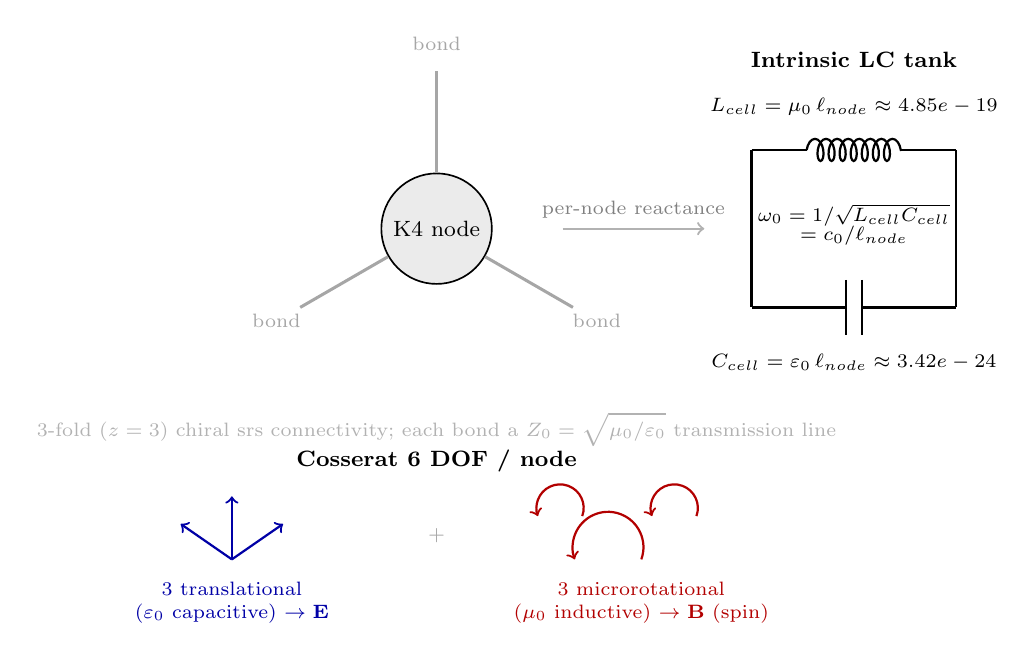
\begin{tikzpicture}[scale=1.0, transform shape,
    dofE/.style={->, thick, blue!65!black},
    dofB/.style={->, thick, red!70!black},
    every node/.style={font=\footnotesize}]

    % --- central node ---
    \node[circle, draw, fill=black!8, minimum size=1.25cm, line width=0.6pt] (node) at (0,0) {K4 node};

    % --- 3-fold (z=3) chiral srs nearest-neighbour bond stubs (trivalent Laves connectivity) ---
    % z=3-diamond -> z=3-chiral-srs restoration (2026-07-04; discharges the af1 figure debt
    % logged in research/2026-07-03_axiom1-dof-restoration_note.md). srs/Sunada-K4 is DEGREE-3;
    % the former 4-stub tetrahedral geometry depicted the doubly-ratified-against z=4 diamond.
    \foreach \ang/\lab in {90/{}, 210/{}, 330/{}} {
        \draw[line width=1.1pt, gray!70] (node) -- (\ang:2.0);
        \node[gray!70, font=\scriptsize] at (\ang:2.35) {bond};
    }
    \node[gray!60, font=\scriptsize, align=center] at (0,-2.55)
        {3-fold ($z=3$) chiral srs connectivity; each bond a $Z_0=\sqrt{\mu_0/\varepsilon_0}$ transmission line};

    % --- intrinsic LC tank (drawn to the right as the node's internal reactance) ---
    \begin{scope}[shift={(5.3,0)}]
        \node[font=\footnotesize\bfseries] at (0,2.15) {Intrinsic LC tank};
        % inductor (coil) top branch
        \draw[line width=0.8pt] (-1.3,1.0) -- (-0.6,1.0);
        \draw[line width=0.8pt, decorate, decoration={coil, aspect=0.5, segment length=4pt, amplitude=4pt}]
              (-0.6,1.0) -- (0.6,1.0);
        \draw[line width=0.8pt] (0.6,1.0) -- (1.3,1.0);
        \node[align=center, font=\scriptsize] at (0,1.55) {$L_{cell}=\mu_0\,\ell_{node}\approx\SI{4.85e-19}{\henry}$};
        % capacitor bottom branch
        \draw[line width=0.8pt] (-1.3,-1.0) -- (-0.1,-1.0);
        \draw[line width=0.8pt] (-0.1,-0.65) -- (-0.1,-1.35);
        \draw[line width=0.8pt] (0.1,-0.65) -- (0.1,-1.35);
        \draw[line width=0.8pt] (0.1,-1.0) -- (1.3,-1.0);
        \node[align=center, font=\scriptsize] at (0,-1.7) {$C_{cell}=\varepsilon_0\,\ell_{node}\approx\SI{3.42e-24}{\farad}$};
        % side wires closing the loop
        \draw[line width=0.8pt] (-1.3,1.0) -- (-1.3,-1.0);
        \draw[line width=0.8pt] (1.3,1.0) -- (1.3,-1.0);
        \node[align=center, font=\scriptsize] at (0,0.05)
            {$\omega_0 = 1/\sqrt{L_{cell}C_{cell}}$\\[-1pt] $= c_0/\ell_{node}$};
    \end{scope}
    \draw[->, gray!60, line width=0.8pt] (1.6,0) -- (3.4,0)
        node[midway, above, font=\scriptsize, gray] {per-node reactance};

    % --- the Cosserat 6-DOF split (below) ---
    \begin{scope}[shift={(0,-4.2)}]
        \node[font=\footnotesize\bfseries] at (0,1.25) {Cosserat 6 DOF / node};
        % 3 translational -> E
        \draw[dofE] (-2.6,0) -- (-2.6,0.8);
        \draw[dofE] (-2.6,0) -- (-1.95,0.45);
        \draw[dofE] (-2.6,0) -- (-3.25,0.45);
        \node[blue!65!black, align=center, font=\scriptsize] at (-2.6,-0.55)
            {3 translational\\($\varepsilon_0$ capacitive) $\to \mathbf{E}$};
        % 3 microrotational -> B
        \draw[dofB] (2.6,0) arc (-20:200:0.45);
        \draw[dofB] (1.85,0.55) arc (-20:200:0.30);
        \draw[dofB] (3.3,0.55) arc (-20:200:0.30);
        \node[red!70!black, align=center, font=\scriptsize] at (2.6,-0.55)
            {3 microrotational\\($\mu_0$ inductive) $\to \mathbf{B}$ (spin)};
        \node[gray!70, font=\scriptsize] at (0,0.3) {$+$};
    \end{scope}

\end{tikzpicture}
\caption{K4 node anatomy. Each node of the chiral Laves K4 Cosserat lattice carries one intrinsic electromagnetic LC tank ($L_{cell}=\mu_0\ell_{node}\approx\SI{4.85e-19}{\henry}$, $C_{cell}=\varepsilon_0\ell_{node}\approx\SI{3.42e-24}{\farad}$; \kbleaf{src/ave/core/constants.py} \texttt{L\_CELL}, \texttt{C\_CELL}), resonating at $\omega_0=c_0/\ell_{node}=\sqrt{1/(L_{cell}C_{cell})}\approx\SI{7.76e20}{\radian\per\second}$ (\texttt{OMEGA\_C}), connects to its three nearest neighbours (3-fold $z=3$ chiral srs / Sunada-K4 / Laves connectivity) through $Z_0=\sqrt{\mu_0/\varepsilon_0}=\sqrt{L_{cell}/C_{cell}}\approx376.73\,\Omega$ bond transmission lines, and hosts six Cosserat degrees of freedom: three translational (capacitive $\varepsilon_0$, identified with $\mathbf{E}$) and three microrotational (inductive $\mu_0$, identified with $\mathbf{B}$; the substrate-native origin of intrinsic spin). Axioms~1 (substrate topology). Schematic; not driver-generated.}
\label{fig:vol9_node_anatomy}
\end{figure}
